\documentclass[sigconf]{acmart}
% ===== Don't touch this :) ======
\settopmatter{printacmref=false} % Removes citation information below abstract
\renewcommand\footnotetextcopyrightpermission[1]{} % removes footnote with conference information in first column
\renewcommand\footnotetextauthorsaddresses[1]{}
\pagestyle{plain} % removes running headers
% ================================

\usepackage{graphicx}

% for red coloring
\def\bad#1{\textcolor{red}{#1}}

\begin{document}
\title{CS561 Midway Report: Implementing SIEVE in the Postgres Bufferpool}

\author{Ryan Crosier}
\affiliation{%
    \institution{Boston University}
    \country{}
}
\author{Will Garlington}
\affiliation{%
    \institution{Boston University}
    \country{}
}
\author{Jackson Gilstrap}
\affiliation{%
    \institution{Boston University}
    \country{}
}

\begin{abstract}
    The buffer cache is a key data structure in the DBMS that helps reduce unecessary disk I/Os. Eviction policies help determine when data in a cache is no longer needed and removes it, creating room for new data. Some of the most common algorithms are Least Recently Used (LRU), Least Frequently Used (LFU), First In First Out (FIFO), and many others. PostgreSQL uses the CLOCK \bad{citethis} algorithm, a modification of LRU designed to minimize the overhead of maintaining an ordered list of recently used pages. For our project, we implement SIEVE, an eviction policy originally designed as an LRU alternative for web caches, into PostgreSQL. SIEVE is advantageous due to its lock-less design and its ability to be integrated into existing cache architectures. Whilst SIEVE was originally made for the web, there could be possible use for it in database systems such as PostgreSQL. Our experiments benchmark Sieve against other eviction policies using \textit{pgbench}. We find that SIEVE provides little (if any) improvement in terms of throughput and cache-hit ratio over the default buffer cache eviction policy on mixed and skewed workloads.
\end{abstract}

\maketitle

% =============================================================================
\section{Introduction}
% =============================================================================

\subsection{Motivation}

The most successful cache eviction policy introduced in recent years is SIEVE \cite{SIEVE}, an algorithm which is even simpler to implement than LRU. While originally designed for web-caching workloads, it has been found to be useful in many workloads with a high degree of data skew. While the paper introducing SIEVE concedes that it may not perform well for buffer cache workloads due to the presence of range scans, many real-world workloads may have a much higher proportion of point queries for which the benefits of SIEVE can be exploited.

\subsection{Problem Statement}

The problem we are exploring is whether or not there are workloads for which SIEVE outperforms other simple eviction policies for the bufferpool in PostgreSQL. PostgreSQL uses the CLOCK algorithm for buffer cache eviction by default, and we implement the following policies in addition: LRU, LFU, FIFO \bad{LIST POLICIES HERE}. We will then explore workloads with different data skews and determine whether SIEVE grants any performance benefits or reduces write amplification.

\subsection{Contributions}

We make the following contributions:

\begin{itemize}
    \item We implement a framework in PostgreSQL for implementing and switching between different buffer cache eviction policies at compile time.
    \item We present results indicating that SIEVE does not offer any significant performance benefits over CLOCK in skewed and mixed workloads.
\end{itemize}


% =============================================================================
\section{Background}
% =============================================================================
For decades cache eviction has been primarily dominated by very simple primitive algorithms such as First In First Out(FIFO) and Least Recently Used (LRU). 
More complex algorithms such as Adaptive Replacement Cache (ARC) typically tend to have better results, however require the developer to implement hundreds of lines of code. 
This persistent trade off between simplicity and efficiency has been continuously discussed and researched in system research. 
\cite{SIEVE}SIEVE is a recent advancement in this space, originally designed for and evaluated against web cache workloads. 
The authors categorize SIEVE as a cache eviction primitive similar to LRU or FIFO. Structurally, it is built upon a single FIFO queue and utilizes a "moving hand" pointer to track whether data has been recently accessed. 
This hand scans from the tail toward the head of the queue, resetting the "visited" bit of objects it encounters. An object is only evicted if its visited bit is 0; otherwise, it is retained in its original position, effectively "sifting" the cache to preserve popular data. 

\subsection{Simplicity and Performance}
A primary advantage of SIEVE is its ease of integration; the authors report that it can be implemented within existing production environments using an average of fewer than 20 lines of code changes. 
This simplicity translates directly to high-performance scalability. In multi-threaded environments, SIEVE has demonstrated nearly double the throughput of optimized LRU implementations, 
largely because its "lazy promotion" mechanism requires no locking during cache hits. 

\subsection{Challenges of Scan-Resistence}
While SIEVE excels in web workloads—which typically follow a Power-law (Zipfian) distribution—its application in Relational Database Management Systems (RDBMS) reveals a notable limitation: it is not inherently scan-resistant. 
This vulnerability stems from cache pollution and the absence of a ghost cache. In RDBMS block cache workloads, sequential scans frequently intermingle popular "hot" data with massive volumes of "one-time" scan data. 
Without a ghost cache to track recently evicted items and differentiate them from transient scan results, SIEVE rapidly evicts popular data, effectively neutralizing the algorithm's efficiency gains in these environments.
% =============================================================================
\section{Architecture}
% =============================================================================
We use a new eviction policy framework which routes high level hit, insert, and
invalidate calls from the buffer manager through to methods specific to each
eviction strategy. This approach was chosen with the goal of allowing the eviction
algorithm to be chosen at runtime rather than requiring recompilation of the source
code, or switching between different versions of the codebase.

\subsection{SIEVE Implementation}

Our SIEVE implementation uses two arrays, SieveNext and SievePrev, to track page
positions and emulate a linked list, along with a \emph{head} pointer to manage the 
position of the SIEVE algorithm 'sweep'. Each array is sized according to the
number of buffers configured (NBuffers), where the Nth element of SieveNext and SievePrev
point to the head and tail respectively. During an insertion or invalidation,
the \emph{head} is set as needed, and SieveNext and SievePrev values are
updated to reflect the new ordering of the list.

\subsection{Benchmark Explanations}

To benchmark our changes, we are starting with synthetic benchmarks built using Postgres' built-in program \textit{pgbench} (also used for benchmarks in~\cite{ACE}). We use simple select and update queries, which can each be independently weighted to change the workload skew.

We are interested in evaluating the impact of three variables: workloads skew, data skew, and buffer size. To skew the workload, we give different weights to our select and update scripts in \textit{pgbench}. To skew data access, we compare queries drawn from Zipfian and uniform distributions. Finally, we vary buffer size between 8MB and 128MB.

Because the Shared Computing Cluster (SCC) has routine downtime and does not offer details on the internal hardware, we have chosen to benchmark on a mid-range consumer desktop owned by one of the authors. The system has 32GB of DDR4 RAM, an AMD Ryzen 5600X 6-Core CPU with a base clock speed of 3.7GHZ, and a 240GB SATA SSD.

% =============================================================================
\section{Results}
% =============================================================================
The default bufferpool size in Postgres is 128MB, so we start by evaluating the difference between SIEVE and the default Clocksweep implementation with this buffer size. As shown in Figures \bad{fill this in}, the performance difference between the implementations is negligible for both uniform and Zipfian distributions. Moving to an 8MB bufferpool, we see that the the trend continues.

\begin{figure}[ht]
    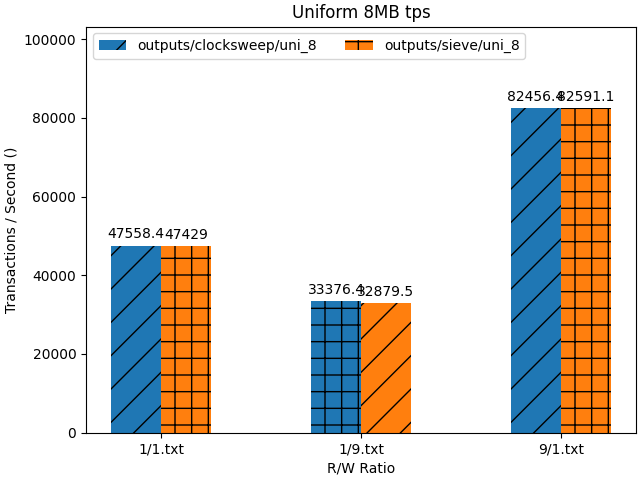
\includegraphics[width=4cm]{images/uniform_8mb_tps.png}
    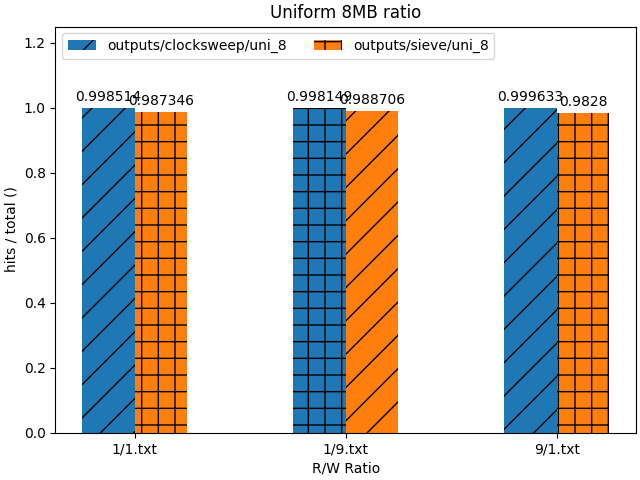
\includegraphics[width=4cm]{images/uniform_8mb_cache.png}
    \caption{Uniform queries with 8MB Cache}
\end{figure}
\begin{figure}[ht]
    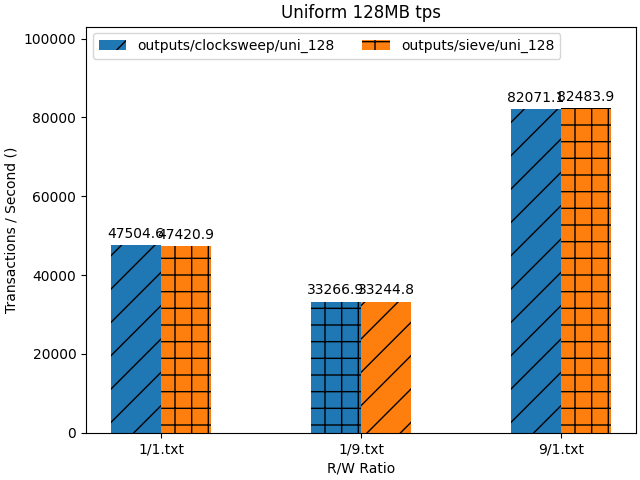
\includegraphics[width=4cm]{images/uniform_128mb_tps.png}
    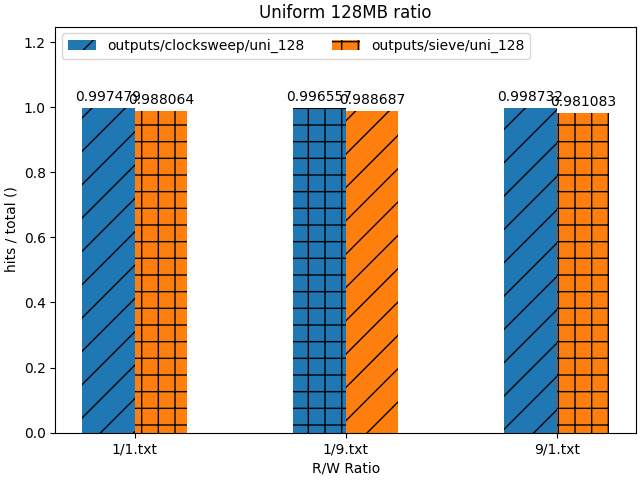
\includegraphics[width=4cm]{images/uniform_128mb_cache.png}
    \caption{Uniform queries with 128MB Cache}
\end{figure}
\begin{figure}[ht]
    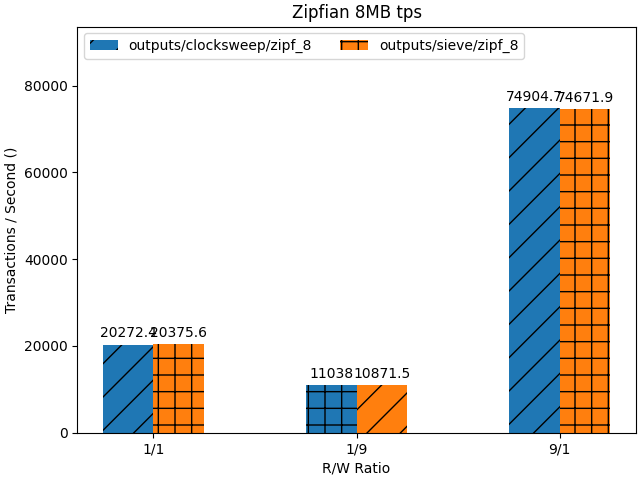
\includegraphics[width=4cm]{images/zipf_8mb_tps.png}
    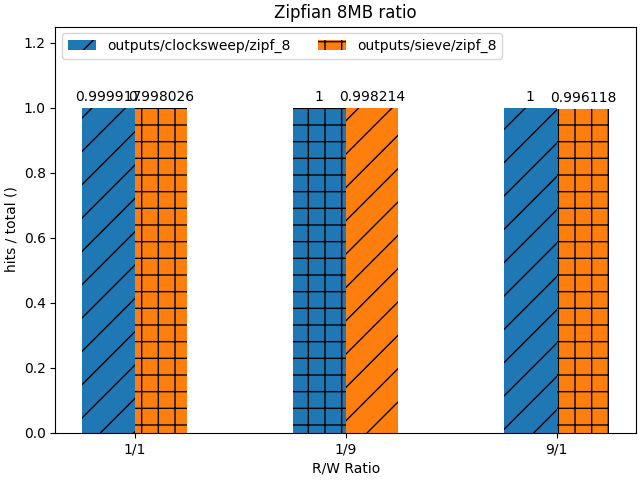
\includegraphics[width=4cm]{images/zipf_8mb_cache.png}
    \caption{Zipfian queries with 8MB Cache}
\end{figure}
\begin{figure}[ht]
    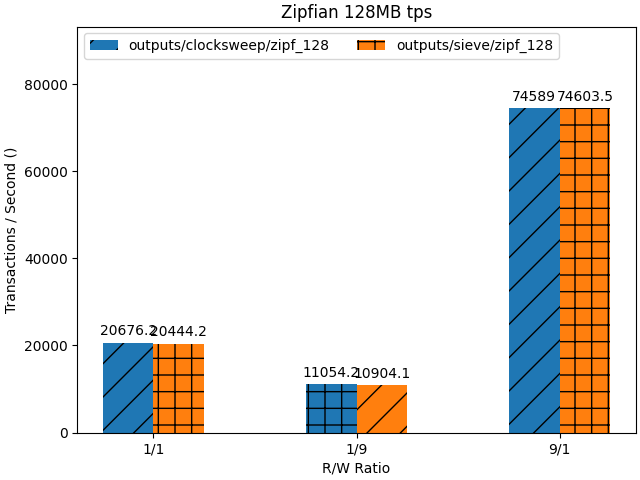
\includegraphics[width=4cm]{images/zipf_128mb_tps.png}
    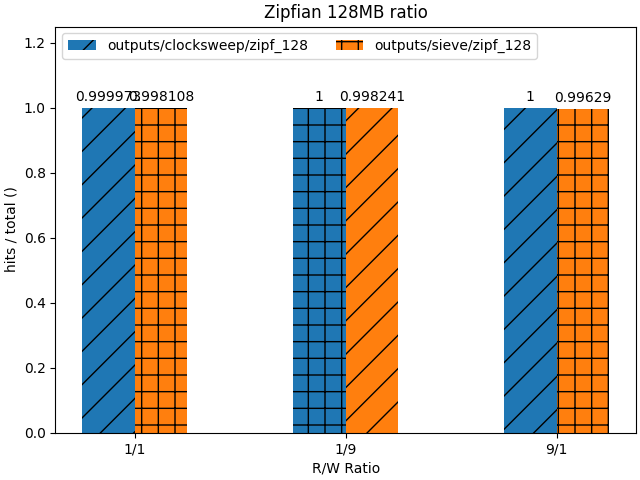
\includegraphics[width=4cm]{images/zipf_128mb_cache.png}
    \caption{Zipfian queries with 128MB Cache}
\end{figure}


% =============================================================================
\section{Conclusion}
% =============================================================================

We have implemented and evaluated SIEVE against Clock Sweep for various synthetic workloads and found that there is little difference in throughput and cache hit ratio. Our next steps are to additionally measure the write amplification of different eviction policies over different workloads and determine if SIEVE is able to pull ahead in any of those scenarios. We would also like to test synthetic workloads include range scans, which should perform worse according to~\cite{SIEVE}.


% reference
{
    \bibliographystyle{ACM-Reference-Format}
    \bibliography{biblio}
} 

\end{document}
